\section{Generación de Lenguaje Natural}\label{s:nlg}
Como se ha descrito y observado gracias a la tabla \ref{tab:dailymail}, el tráfico de correos electrónicos diarios continúa en constante crecimiento hasta llegar, al menos, a la gigantesca cifra de 376 mil millones enviados al día en todo el mundo. Esto se revierte en una gran cantidad de tiempo invertido para la redacción de todos estos mensajes que no se mandan de manera automática. Sin embargo, esta gran dedicación al e-mail lleva produciéndose desde hace más de una década, cuando no nos encontrábamos con cifras de tráfico tan elevadas. Según \cite{mckinsey}, de media los empleados invertían el 28\% de su tiempo semanal en la gestión del correo electrónico (como viene reflejado en la figura \ref{fig:e-mailwork}). Esto se traduce en más de once horas dedicadas única y exclusivamente a leer y contestar mensajes, enviando y recibiendo una media de 124 e-mails por día \citep{radicati2015email}. Por si estos datos no fueran suficientemente preocupantes, de cara a la productividad laboral y resolución eficiente de las tareas, según \cite{forbes} este problema se ha agravado en los últimos años por diversas causas (entre las que se encuentra la pandemia de la Covid-19). En definitiva, hoy en día podemos afirmar que tanto en el ámbito profesional como personal se invierte una gran cantidad de esfuerzo y tiempo para gestionar nuestra cuenta de e-mail, lo cual plantea un problema en el que vemos que, en lugar de ser una herramienta útil, se convierte en una responsabilidad más que debe llevarse al día y de la que no es posible desprenderse ya que la capacidad de mandar estos mensajes es imprescindible para llevar a cabo tareas del día a día. Pero, ¿y si fuera posible ahorrar todo este tiempo de escritura de correos electrónicos?

\begin{figure}[h]
	\centering%
	\centerline{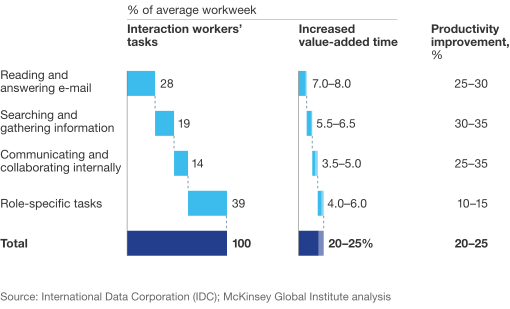
\includegraphics[width = 0.9\textwidth]{Imagenes/Bitmap/mckinsey.png}}%
	\caption{Porcentaje de tiempo de un trabajador dedicado a cada tarea}%
	\label{fig:e-mailwork}
\end{figure}

Para lograr este propósito es imprescindible profundizar en la rama de la Inteligencia Artificial conocida como \textit{Generación de Lenguaje Natural} (cuyas siglas son \textit{NLG} por su nombre en inglés \textit{Natural Language Generation}). Un buen ejemplo de aplicación de las técnicas de generación automática de textos son los 100.000 libros que Philip M. Parker puso a la venta en la plataforma \textit{Amazon.com} incluyendo títulos de temáticas tan variadas como \textit{El libro oficial del paciente sobre la estenosis espinal} \citep{parker2002official}, \textit{Perspectivas mundiales de 2009 a 2014 de los envases de 60 miligramos de Fromage Frais} \citep{parkerfromage},  \textit{Perspectivas de 2007 a 2012 de las tapetes de nudo, alfombras de baño y conjuntos que miden 6 pies por 9 pies o menos en la India} \citep{parkerrugs} y \textit{Tesauro Quechua - Inglés} \citep{parkerquechua}.

Resulta evidente que dicha cantidad de libros no pudieron ser escritos por Parker, sino que debió hacerse uso de técnicas de generación automática de textos. El algoritmo utilizado para dicho propósito, se engloba dentro de los métodos de generación conocidos como \textit{text-to-text} (texto a texto en castellano), dado que este tipo de técnicas toman como entrada textos ya existentes (normalmente escritos a mano y no generados automáticamente) y producen un nuevo texto coherente como salida. Otras aplicaciones de este tipo de métodos son la traducción automática de un idioma a otro \citep{hutchins2009introduction, oettinger2013automatic}, el resumen automático de textos \citep{mani2001automatic, nenkova2011automatic}, la simplificación de textos complejos, ya sea para hacerlos más accesibles para un público de lectores de bajo nivel de alfabetización \citep{siddharthan2014survey, bautista2011empirical} o niños \citep{macdonald2016summarising}, corrección automática de ortografía, gramática y texto \citep{kukich1992techniques, ng2014conll}, generación automática de revisiones de artículos científicos \citep{bartoli2016your}, generación de paráfrasis dada una frase de entrada \citep{bannard2005paraphrasing}, generación automática de preguntas con fines didácticos y educativos \citep{brown2005automatic}, generación automática de relatos dada una descripción conceptual de la historia deseada \citep{gervas2004story} o reescritura de textos (en concreto correos electrónicos) con estilo en función del destinatario \citep{mitfg}.

Además de estos métodos text-to-text, existen los llamados \textit{data-to-text} (datos a texto), en los cuales en lugar de recibir un texto como entrada, se genera el lenguaje a partir de datos. Estos pueden ser de todo tipo para dar lugar a informes o resúmenes como pueden ser de índole climatológica \citep{goldberg1994using, ramos2014linguistic}, financiera \citep{plachouras2016interacting}, ingenieril, como por ejemplo el trabajo desarrollado por \cite{yu2007choosing} para generar resúmenes de datos recopilados por sensores en turbinas de gas, sanitaria \citep{huske2003text, banaee2013towards}, como la investigación llevada a cabo por \cite{portet2009automatic} para obtener informes textuales a partir de datos de cuidados intensivos neonatales, o, incluso, deportivos \citep{theune2001data, chen2008learning}. Además de informes o resúmenes, también se utilizan los métodos \textit{data-to-text} para otros propósitos como la composición de discursos narrativos para relatos de varios personajes a partir de partidas de ajedrez \citep{gervas2014composing}, redacción de periódicos electrónicos a partir de datos de sensores \citep{molina2011generating}, generación de texto que aborda problemas medioambientales como el seguimiento de la fauna \citep{siddharthan2012blogging, ponnamperuma2013tag2blog}, la información medioambiental personalizada \citep{wanner2015getting} y la mejora del compromiso de los ciudadanos científicos a través de los comentarios generados \citep{van2016role} o producción de información interactiva sobre artefactos culturales \citep{stock2007adaptive}, entre otros.

Debido a que el objetivo de este trabajo se centra en la generación de correos electrónicos a partir del asunto, exploraremos en detalle las técnicas de Generación de Lenguaje Natural y, en especial, los métodos text-to-text. Para profundizar en los algoritmos y arquitecturas empleados ante los problemas de tipo data-to-text, conviene consultar la investigación llevada a cabo por \cite{gatt2018survey}, en la cual muestran el estado del arte de los trabajos realizados en este ámbito.

\subsection{¿Qué es la Generación de Lenguaje Natural?}
Dado que tanto los sistemas text-to-text como data-to-text y todas sus aplicaciones mencionadas anteriormente pertenecen a la rama de Generación de Lenguaje Natural, esta no debe definirse en función de la entrada del sistema, sino en la salida. Según \cite{biblia} la NLG es la conceptualización del ``campo de la inteligencia artificial y la lingüística computacional que se centra en los sistemas informáticos que son capaces de producir textos comprensibles en inglés u otra lengua humana. [...] Como área de investigación, la NLG presenta una perspectiva única ante problemas fundamentales de la inteligencia artificial, la ciencia cognitiva y la interacción. Estos incluyen cuestiones como por ejemplo cómo deben ser representados y cómo debe razonarse con la lingüística y el dominio del conocimiento, qué significa que un texto esté correctamente redactado y cómo es la mejor forma de comunicar información entre las computadoras y los usuarios.'' Por lo tanto, la Generación de Lenguaje Natural se puede definir como el ámbito que engloba el estudio de la producción de lenguaje no artificial, así como el diseño e implementación de algoritmos y sistemas computacionales cuyo resultado debe ser un texto que imite la forma en que los humanos se comunican verbalmente \citep{vicente2015generacion}, ya sea oralmente o por escrito \citep{del2007que}. Es decir, independientemente de la entrada recibida, se precisa el significado de NLG a partir de la salida esperada por el problema planteado. Tanto es así, que, como hemos visto, la entrada del sistema puede variar excesivamente \citep{mcdonald1993issues}: desde textos (que son precisamente los sistemas text-to-text) hasta datos de todo tipo como partidas de ajedrez \citep{gervas2014composing}, pictogramas \citep{gonzalez2019traductor} e, incluso, vídeos \citep{thomason2014integrating}. Sin embargo, autores como \cite{duvsek2020evaluating} acotan la definición de los sistemas de NLG estableciendo que la entrada deben ser representaciones semánticas, obviando así la primera tarea de la arquitectura propuesta por \cite{biblia} conocida como macro planificación o determinación del contenido (se explicará en la sección \textcolor{red}{poner nº}), que es precisamente el punto en el que se generan dichas representaciones semánticas.

Cabe destacar que, aunque desde un principio hayamos diferenciado entre métodos text-to-text y data-to-text, ni los límites entre las dos aproximaciones ni la pertenencia de algunas técnicas a ellas se encuentran claramente definidos. Un ejemplo de ello podemos encontrarlo en la generación automática de resúmenes de textos. En principio se caracterizaría claramente como un sistema text-to-text. No obstante, al hacer frente a este problema se han desarrollado soluciones con las conocidas técnicas abstractivas \citep{genest2011framework}, que, como explican \cite{hahn2000challenges}, a diferencia de los métodos de extracción evitan recoger las frases completas y se limitan a tomar unidades semánticas. Este tipo de técnicas usadas, por ejemplo, en la obtención de opiniones de reseñas para la posterior generación de frases nuevas \citep{labbe2012towards}, también provienen de problemas data-to-text. A la inversa, un sistema data-to-text puede hacer uso de técnicas que principalmente son utilizadas en los casos de uso text-to-text \citep{mcintyre2009learning, kondadadi2013statistical}. Por otro lado, podría parecer que los métodos de \textit{deep learning} \citep{goodfellow2016deep} deben ser mayoritariamente utilizados en los problemas data-to-text utilizando el trabajo llevado a cabo por \cite{mikolov2013efficient}. Sin embargo, se han desarrollado extensamente esta clase de soluciones para la NLG con gran variedad de arquitecturas como las redes neuronales recurrentes \citep{cho2014learning, tang2016context} muy a menudo combinadas con la memoria a corto plazo o LSTM \citep{chen2016enhanced}.
